\chapter{Численный метод для вариационной постановки задачи переноса излучения}

Самосопряженные задачи в вариационной постановке весьма удобны для построения численных методов. При этом построенные методы сохраняют самосопряженность разностного оператора, даже на неструктурированных сетках. 

\section{Метод Ритца}

В основе метода Ритца \cite{marchuk1981} лежит идея замены исходной задачи минимизации функционала $\mathcal{G}(\varphi)$ в пространстве $\mathfrak{H}_0$ на задачу минимизации этого же функционала в конечномерном подпространстве $\mathcal{H}_0 \subset \mathfrak{H}_0$. При этом решение разлагается по базису $\psi_i(\vec r, \vec \Omega)$ пространства $\mathcal{H}_0$:
\[
\varphi(\vec r, \vec \Omega) = \sum_i \varphi_i \psi_i(\vec r, \vec \Omega).
\]
Подставляя это выражение в задачу \eqref{eq:variational} минимизации $\mathcal{G}(\varphi)$
\[
\mathcal{G}(\varphi) = [\varphi, \varphi] - 2 (\varphi, I_\text{p}) \to \min_{\varphi \in \mathcal{H}_0}
\label{eq:minimize}
\]
и пользуясь линейностью скалярных произведений, имеем
\[
\sum_{i,j} \varphi_{i}\varphi_{j} [\psi_i, \psi_j] - 2 \sum_{j} \varphi_i(\psi_i, I_\text{p})\to \min_{\varphi \in \mathcal{H}_0}.
\]
Эта задача является задачей минимизации квадратичной формы и сводится к системе линейных уравнений
\begin{equation*}
\sum_{j} [\psi_i, \psi_j] \varphi_j = (\psi_i, I_\text{p}), \qquad i = 1, 2, \dots, \operatorname{dim} \mathcal{H}_0.
\end{equation*}

На практике удобно выбрирать базис пространства $\mathcal{H}_0$ в виде прямого произведения базиса в координатном пространстве и базиса в угловом пространстве:
\begin{gather}
\varphi(\vec r, \vec \Omega) = \sum_k \varphi_{k}(\vec r)\theta_k(\vec \Omega)\\
\varphi_k(\vec r) = \sum_i \varphi_{i,k} \phi_i(\vec r)\\
\psi_{i,k}(\vec r, \vec \Omega) = \phi_i(\vec r) \theta_k (\vec \Omega).
\label{eq:discrete}
\end{gather}
Отметим, что в силу четности $\varphi$ по $\vec \Omega$ в качестве $\theta_k(\vec \Omega)$ разумно выбирать также четные функции.

\subsection{Угловая дискретизация}

Подставим представление \eqref{eq:discrete} базисных функций в скалярное произведение $(\psi_{i,k}, \psi_{i',k'})$:
\begin{multline*}
(\psi_{i,k}, \psi_{i',k'}) = \iint\limits_{G \times 4\pi} 
\varkappa(\vec r) \phi_i(\vec r) \theta_k(\vec \Omega)\phi_{i'}(\vec r)  \theta_{k'}(\vec \Omega) d\vec r d\Omega = \\ =
\int\limits_{4\pi} \theta_k(\vec \Omega) \theta_{k'}(\vec \Omega) d\Omega
\int\limits_G \varkappa(\vec r) \phi_i(\vec r) \phi_{i'}(\vec r) d\vec r.
\end{multline*}
Обозначим первый интеграл от угловых базисных функций через $\mathscr H_{kk'}$:
\[
\mathscr H_{kk'} \equiv \int\limits_{4\pi} \theta_k(\vec \Omega) \theta_{k'}(\vec \Omega) d\Omega.
\]
Данная матрица зависит только от углового базиса, и, при необходимости, может быть сделана единичной путем ортогонализации базиса, например, с помощью процедуры Грама-Шмидта \cite{beklemishev1998}.

Аналогичным образом найдем скалярное произведение $\left(\frac{1}{\varkappa} \vec\Omega\nabla \psi_{i,k}, \frac{1}{\varkappa}\vec\Omega\nabla\psi_{i',k'}\right)$:
\begin{multline*}
\left(\frac{1}{\varkappa} \vec\Omega\nabla \psi_{i,k}, \frac{1}{\varkappa}\vec\Omega\nabla\psi_{i',k'}\right) = \iint\limits_{G \times 4\pi} 
\frac{1}{\varkappa(\vec r)} \Omega_\alpha \nabla_\alpha\phi_i(\vec r) \theta_k(\vec \Omega) \Omega_\beta \nabla_\beta\phi_{i'}(\vec r)  \theta_{k'}(\vec \Omega) d\vec r d\Omega = \\ =
\int\limits_{4\pi} \Omega_\alpha \Omega_\beta\theta_k(\vec \Omega) \theta_{k'}(\vec \Omega) d\Omega
\int\limits_G \frac{1}{\varkappa(\vec r)} \left[\nabla_\alpha \phi_i(\vec r)\right] \left[\nabla_\beta \phi_{i'}(\vec r)\right] d\vec r.
\end{multline*}
Обозначим интеграл от угловых функций через $\mathscr{K}^{\alpha\beta}_{kk'}$:
\[
\mathscr{K}^{\alpha\beta}_{kk'} \equiv \int\limits_{4\pi} \Omega_\alpha \Omega_\beta \theta_k(\vec \Omega) \theta_{k'}(\vec \Omega) d\Omega.
\]

То же самое проделаем с интегралом
%\begin{multline*}
\[
\iint\limits_{\partial G \times 4\pi} |(\vec \Omega \vec n)| \psi_{i,k}\psi_{i',k'} d\Omega d \Gamma = 
\int\limits_{\partial G} \left[\int\limits_{4\pi} \left|\big(\vec \Omega \vec n(\vec r)\big)\right|
\theta_k(\vec \Omega) \theta_{k'}(\vec \Omega) d\Omega\right] \phi_i(\vec r) \phi_{i'}(\vec r) d\Gamma
\]
%\end{multline*}
В отличие от двух предыдущих случаев данный интеграл не представляется в виде произведения двух интегралов от угловой и пространственной части, так как вектор нормали $\vec n$ зависит от положения точки $\vec r$ на границе $\partial G$. Обозначим величину в квадратных скобках через $\mathscr{B}_{kk'}(\vec n)$:
\[
\mathscr{B}_{kk'}(\vec n) = \int\limits_{4\pi} \left|\big(\vec \Omega \vec n\big)\right|
\theta_k(\vec \Omega) \theta_{k'}(\vec \Omega) d\Omega.
\]
Пользуясь четностью угловых функций $\theta_k(\vec \Omega)$ это выражение можно записать в эквивалентной форме
\[
\mathscr{B}_{kk'}(\vec n) = \int\limits_{(\vec \Omega \vec n) > 0} \big(\vec \Omega \vec n\big)
\theta_k(\vec \Omega) \theta_{k'}(\vec \Omega) d\Omega.
\]

В случае, если граница области $\partial G$ состоит из небольшого количества многоугольников (например, $G$ --- куб), существует лишь несколько различных вариантов для матрицы $\mathscr{B}_{kk'}$. К тому же, данные матрицы совпадают для нормалей, отличающихся лишь знаком.

Найдем также выражение для линейного слагаемого в функционале $\mathcal{G}(\varphi)$:
\begin{multline*}
(\psi_{i,k}, I_\text{p}) = \iint\limits_{G \times 4\pi} \varkappa(\vec r) \phi_i(\vec r) \theta_k(\vec \Omega) I_\text{p} (\vec r, \vec \Omega) d\vec r d\vec \Omega = \\ =
\int\limits_{G} \varkappa(\vec r) \phi_i(\vec r) \left[
\int\limits_{4\pi} \theta_k(\vec \Omega) I_\text{p}(\vec r, \vec \Omega) d\Omega
\right] d\vec r
\end{multline*}
и обозначим
\[
\mathscr{R}_{k}(\vec r) = \int\limits_{4\pi} \theta_k(\vec \Omega) I_\text{p}(\vec r, \vec \Omega) d\Omega.
\]

Принимая правило суммирования по повторяющемуся индексу, задача минимизации может быть записана в следующем дискретизированном по угловой переменной виде
\begin{multline*}
\mathscr H_{kk'} \int\limits_{G} \varkappa \varphi_k \varphi_{k'} d\vec r +
\mathscr K_{kk'}^{\alpha\beta} \int\limits_{G} \frac{1}{\varkappa} [\nabla_\alpha \varphi_{k}] [\nabla_\beta \varphi_{k'}] d\vec r +
\int\limits_{\partial G} \mathscr B_{kk'}(\vec n) \varphi_{k}\varphi_{k'} d\Gamma - \\ - 2 \int\limits_{G}
\varkappa \varphi_k \mathscr{R}_k d\vec r \to \min_{\varphi_k}.
\end{multline*}

Данная задача соответствует вариационной постановке для системы из $K = \operatorname{dim} \left\{\theta_k(\vec \Omega)\right\}$ связанных эллиптических уравнений для функций $\varphi_k(\vec r)$.

\subsection{Пространственная дискретизация}

Функции $\varphi_k(\vec r)$ и, как следствие, $\phi_i(\vec r)$ должны принадлежать классу функций, имеющих обобщенную первую производную, так как
\[
\mathcal{H}_0 \subset \mathfrak{H}_0 \subset H^1(G).
\]

Пусть в области $G$ построена триангуляция $\mathcal{T} = \left\{T_i\right\}_{i=1}^N$:
\[
G = \bigcup_{i=1}^{N} T_i, \quad T_i \cap T_j = \partial T_i \cap \partial T_j, \; i \neq j.
\]
Потребуем, чтобы $\varphi_k(\vec r)$ были линейными функциями координат $\vec r$ в каждом элементе триангуляции $T_j$. Тогда требование $\varphi_k(\vec r) \in H^1(G)$ накладывает на $\varphi_k(\vec r)$ дополнительно требование непрерывности. Таким образом, $\varphi_k(\vec r)$ --- кусочно линейные функции координат $\vec r$, причем на каждом элементе $T_j$ функция является линейной. Обозначим пространство таких функций как $\mathcal{P}_1(T_j)$. Такие функции однозначно восстанавливаются по своим значениям в узлах триангуляции. При этом функции $\phi_i(\vec r)$ можно определить как кусочно-линейные функции с минимальным носителем, удовлетворяющие условию $\phi_i(\vec r_i) = 1$. При этом носитель функции $\phi_i(\vec r)$ равен
\[
\operatorname{supp} \phi_i(\vec r) = \bigcup_{T_j \ni \vec r_i } T_j.
\]
При таком определение коэффициенты $\varphi_{i,k}$ в разложении
\[
\varphi_k(\vec r) = \sum_{i} \varphi_{i,k} \phi_i(\vec r)
\]
приобретают смысл значений функции $\varphi_k(\vec r)$ в точках $\vec r_i$.

Построим явное выражение для оператора линейной системы
\[
[\mathcal{A} \varphi]_{i,k} \equiv [\phi_i(\vec r)\theta_k(\vec \Omega), \varphi(\vec r, \vec \Omega)].
\]
Пользуясь введенными ранее обозначениями
\begin{equation}
\begin{aligned}
[\mathcal{A} \varphi]_{i,k} &= \mathscr H_{kk'} \int\limits_{G} \varkappa \phi_i \varphi_{k'} d\vec r + {}\\
&{}+ \mathscr K_{kk'}^{\alpha\beta} \int\limits_{G} \frac{1}{\varkappa} [\nabla_\alpha \phi_{i}] [\nabla_\beta \varphi_{k'}] d\vec r +{}\\
&{}+ \int\limits_{\partial G} \mathscr B_{kk'}(\vec n) \phi_{i}\varphi_{k'} d\Gamma.
\end{aligned}
\label{eq:operator}
\end{equation}
При этом правая часть системы $f_{i,k}$ вычисляется как
\begin{equation}
f_{i,k} = (\psi_{i,k}, I_\text{p}) = \int\limits_{G} \phi_i(\vec r) \mathscr R_k(\vec r) d\vec r.
\label{eq:rhs}
\end{equation}
Заметим, что в выражениях \eqref{eq:operator} и \eqref{eq:rhs} интегрирование по всей области $G$ можно заменить на интегрирование по носителю функции $\phi_i(\vec r)$. В свою очередь, носитель данной функции состоит из нескольких сеточных элементов, окружающих узел $\vec r_i$. Учитывая этот факт, запишем оператор в виде
\begin{equation}
\begin{aligned}
[\mathcal{A} \varphi]_{i,k} &= \mathscr H_{kk'} \sum_{T_j \ni \vec r_i}\;\int\limits_{T_j} \varkappa \phi_i \varphi_{k'} d\vec r + {}\\
&{}+ \mathscr K_{kk'}^{\alpha\beta} \sum_{T_j \ni \vec r_i}\;\int\limits_{T_j} \frac{1}{\varkappa} [\nabla_\alpha \phi_{i}] [\nabla_\beta \varphi_{k'}] d\vec r + {}\\
&{}+ \sum_{T_j \ni \vec r_i} \;\int\limits_{\partial G \cap T_j} \mathscr B_{kk'}(\vec n) \phi_{i}\varphi_{k'} d\Gamma\\
f_{i,k} &= \sum_{T_j \ni \vec r_i}\;\int\limits_{T_j} \phi_i(\vec r) \mathscr R_k(\vec r) d\vec r
\end{aligned}
\label{eq:operator2}
\end{equation}

Для того, чтобы вычислить результат применения оператора $\mathcal{A}$ к $\varphi$, достаточно уметь вычислять интегралы по элементам триангуляции $T_j$ от произведения линейных функций и констант.

\section{Квадратурные формулы для вычисления пространственных интегралов}

\subsection{Интеграл по тетраэдру от произведения линейных функций}

При практическом вычислении действия оператора $\mathcal{A}(\cdot)$ на кусочно-линейную функцию $\varphi$ необходимо многократно вычислять
интегралы вида
\begin{equation}
\int\limits_T \varkappa \gamma(\vec r) d \vec r, \quad \gamma(\vec r) = \gamma_1(\vec r)\gamma_2(\vec r),\quad \gamma_{1,2}(\vec r) \in \mathcal{P}_1(T),
\label{eq:vol1}
\end{equation}
когда $T = \operatorname{conv}(\vec r_1,\vec r_2,\vec r_3,\vec r_4)$ --- тетраэдр, а функции $\gamma_{1,2}$ заданы своими значениями в его вершинах. 

Будем искать точную квадратурную формулу для \eqref{eq:vol1}
в виде
\begin{equation}
\int\limits_T \varkappa \gamma(\vec r) d \vec r = \varkappa V \left(w_1 \sum_{j=1}^4 \gamma(\vec r_j) + w_2 \gamma(\vec r_c)\right),
\quad \vec r_c = \frac{\sum_{j=1}^4 \vec r_j}{4}
\label{eq:quad1}
\end{equation}
Из теоремы Соболева \cite{Sobolev1962} следует, что для того, чтобы квадратурная формула, инвариантная относительно действия группы $G$, была точна для всех многочленов степени не выше $n$, она должна быть точна для всех инвариантных относительно $G$ многочленов, степени не выше $G$. В данном случае $G$ --- группа вращений правильного тетраэдра. Поэтому, достаточно проверить, что формула \eqref{eq:quad1} точно интегрирует функции $\gamma \equiv 1$ и $\gamma = (\vec r - \vec r_c)^2$ в правильном тетраэдре.

Из условия точности квадратурной формулы для $\gamma = 1$ получаем
\[
4w_1 + w_2 = 1,
\]
а из условия точности для $\gamma = (\vec r - \vec r_c)^2$ получаем
\[
w_1 = \frac{1}{20}.
\]
При этом $w_2 = \frac{4}{5}$. Итоговая формула имеет вид
\begin{equation}
\int\limits_T \varkappa \gamma(\vec r) d \vec r = \varkappa V \left(\frac{1}{20} \sum_{j=1}^4 \gamma(\vec r_j) + \frac{4}{5} \gamma(\vec r_c)\right).
\label{eq:quad1n2}
\end{equation}
Пусть $\gamma_1(\vec r) = \phi_q(\vec r)$. Тогда $\gamma_1(\vec r_j) = \delta_j^q$
\begin{equation}
\int\limits_T \varkappa \phi_q(\vec r) \gamma_2(\vec r) d \vec r = \frac{\varkappa V}{20} \left(\gamma_2(\vec r_q) + \sum_{j=1}^4\gamma_2(\vec r_j)\right).
\label{eq:quad1n3}
\end{equation}
В последней формуле учтено, что $\phi_q(\vec r_c) = \frac{1}{4}, \gamma_2(\vec r_c) = \frac{1}{4}\sum_{j=1}^4 \gamma_2(\vec r_j)$. Также отметим, что
$\varkappa$ и $V$ входят в формулу только в виде произведения $\varkappa V$.

\subsection{Интеграл по тетраэдру от произведения градиентов линейных функций}

Перейдем к интегралу
\begin{equation}
\int\limits_T \frac{1}{\varkappa} \nabla_\alpha\gamma_1(\vec r)\nabla_\beta\gamma_2(\vec r) d \vec r, \quad \gamma_{1,2}(\vec r) \in \mathcal{P}_1(T),
\label{eq:vol2}
\end{equation}
Поскольку функции $\gamma_{1,2}$ линейны, их производные являются константами.
\begin{equation}
\int\limits_T \frac{1}{\varkappa} \nabla_\alpha\gamma_1(\vec r)\nabla_\beta\gamma_2(\vec r) d \vec r = 
\frac{V}{\varkappa} \nabla_\alpha\gamma_1(\vec r)\nabla_\beta\gamma_2(\vec r)
\label{eq:quad2}
\end{equation}
Пусть $\gamma_1(\vec r) = \phi_q(\vec r)$. Градиент $\phi_q$ направлен вдоль высоты, опущенной из вершины $\vec r_q$ на основание тетраэдра.
Модуль градиента $|\grad \phi_q|$ равен $\frac{1}{h}$, где $h$ --- длина высоты. Учитывая, что объем $V$, длина высоты $h$ и площадь
основания $S$ тетраэдра связаны соотношением $V = \frac{1}{3}S h$, можно заключить, что
\begin{equation}
\operatorname{grad} \phi_q = -\frac{S_q\vec n_q}{3V},
\label{eq:grad}
\end{equation}
где $\vec n_q$ --- внешняя нормаль к грани, противоположной вершине $\vec r_q$, $S_q$ --- площадь этой грани. 
Обозначим\footnote{В этом подразделе под $\vec S$ будет подразумеваться векторная площадь, а не вектор Пойтинга} 
$\vec S^q \equiv S_q \vec n_q$. Данный вектор по модулю равен площади грани и направлен вдоль ее внешней нормали. Таким образом,
\begin{equation}
\nabla_\alpha \phi_q = -\frac{\vec S^q_\alpha}{3V},
\label{eq:nabla}
\end{equation}
Разложим $\gamma_2(\vec r)$ по базисным функциям $\phi$:
\begin{align}
\gamma_2(\vec r) = \sum_{j=1}^4 \phi_j(\vec r) \gamma_2^j\\
\nabla_\beta\gamma_2(\vec r) = \sum_{j=1}^4 \nabla_\beta\phi_j(\vec r) \gamma_2^j = - \sum_{j=1}^4 \frac{\gamma_2^j\vec S^j_\beta}{3V}
\label{eq:nabla2}
\end{align}
Воспользуемся этой формулой для вычисления интеграла
\begin{equation}
J_{\alpha\beta} = \int\limits_T \frac{1}{\varkappa} \nabla_\alpha \phi_q(\vec r) \nabla_\beta \gamma_2(\vec r) d\vec r = 
\frac{V}{\varkappa} \frac{\vec S^q_\alpha}{3V}\sum_{j=1}^4 \frac{\gamma_2^j\vec S^j_\beta}{3V} = 
\frac{1}{9\varkappa V} \vec S_\alpha^q\sum_{j=1}^4 \gamma_2^j\vec S_\beta^j
\label{eq:int2}
\end{equation}
Отметим, что и в этот интеграл $\varkappa$ и $V$ входят в виде произведения $\varkappa V$. Тензор $J_{\alpha\beta}$ 
является тензорным произведением двух векторов $\xi_\alpha \eta_\beta$, причем $\xi_\alpha$ зависит только от точки $\vec r_q$ и 
тетраэдра $T$. Вектор $\eta_\beta$ определяется значениями $\gamma_2(\vec r)$ в вершинах тетраэдра и самим тетраэдром $T$.

\section{Квадратурные формулы для вычисления угловых интегралов}

Для вычисления угловых интегралов
\[
\int\limits_{4\pi} f(\vec \Omega) d\Omega 
\]
в работе применялись квадратурные формулы Лебедева \cite{lebedev}, точные для сферических функций вплоть до $131$-го порядка. Данные формулы являются асимптотически оптимальными относительно коэффициента эффективности
\[
\eta = \frac{(n+1)^2}{3N},
\]
где $n$ --- алгебраическая степень квадратуры, $N$ --- порядок квадратуры (число узлов). Для квадратур гауссового типа $\eta = 1$. Асимптотическая оптимальность означает, что $\eta \to 1$ при $n \to \infty$. Для $n = 131$ квадратурная формула имеет эффективность $\eta \approx 0.99966$.

Отметим, что сферические функции $Y_{l,m}(\vec \Omega)$ могут быть представлены в виде однородных многочленов степени $m$ от $\Omega_x, \Omega_y, \Omega_z$ на единичной сфере (см. приложение \ref{chap:spher}).

Наиболее точная из этих формул использовалась для приближенного интегрирования угловых функций в случае радиального базиса $\theta_k(\vec \Omega)$.

Интегралы по угловой переменной, возникающие при вычислении матриц $\mathscr H_{kk'}, \mathscr K_{kk'}^{\alpha\beta}$, могут быть однократно посчитаны и затабулированы для каждого используемого базиса. Напротив, интегралы, возникающие при вычислении $\mathscr{B}_{kk'}(\vec n)$ зависят от вектора нормали и могут быть затабулированы лишь для простых областей, например, куба, с небольшим числом разных нормалей. Для вычисления таких интегралов предлагается пользоваться квадратурными формулами в каждой точке границы. Так как подынтегральная функция в 
\[
\int\limits_{4\pi} |\vec \Omega \vec n| \theta_k(\vec \Omega) \theta_{k'}(\vec \Omega) d\Omega
\]
из-за модуля содержит особенность производной, использование квадратурных формул Лебедева приводит к возникновению ошибки, значительной даже при использовании самой точной (и самой трудоемкой) из имеющихся квадратурных формул для сферы.

\subsection{Построение квадратурной формулы для полусферы}

Рассмотрим задачу построения квадратурной формулы для интеграла
\begin{equation}
\int\limits_{4\pi} |\vec \Omega \vec n| f(\vec \Omega) d\Omega,
\label{eq:abs}
\end{equation}
точную для всех многочленов $f(\vec \Omega)$ до определенной степени.

Заметим, что благодаря симметрии относительно замены $\vec \Omega \to -\vec \Omega$ интеграл \eqref{eq:abs} может быть записан как интеграл по полусфере $\vec \Omega \vec n > 0$:
\[
\int\limits_{4\pi} |\vec \Omega \vec n| f(\vec \Omega) d\Omega = 
\int\limits_{4\pi} |\vec \Omega \vec n| \frac{f(\vec \Omega) + f(-\vec \Omega)}{2} d\Omega = 
2\int\limits_{(\vec \Omega \vec n) > 0} (\vec \Omega \vec n)\frac{f(\vec \Omega) + f(-\vec \Omega)}{2} d\Omega.
\]
Далее, будем рассматривать интеграл вида
\[
\int\limits_{(\vec \Omega \vec n) > 0} (\vec \Omega \vec n)f(\vec \Omega) d\Omega,
\]
который поворотом координат легко сводится к интегралу по <<северной>> полусфере
\[
I = \iint\limits_{\substack{z > 0\\x^2 + y^2 + z^2 = 1}} f(x, y, z) z dS.
\]
Группами симметрии данного интеграла являются группы вращения $C_n$ относительно оси $Oz$. Будем строить квадратурную формулу, допускающую ту же группу $C_n$.
Для этого расположим узлы квадратуры на окружностях $O_j$, заданных уравнениями
\[
\theta = \theta_j, \quad \varphi = \frac{2\pi k}{n}, k \in 0, 1, \dots, n - 1.
\]
При этом квадратурная формула будет иметь ту же структуру, что и повторный интеграл
\[
I = \int\limits_0^{\pi / 2} \int\limits_0^{2\pi} f(\sin \theta \cos \varphi, \sin \theta \sin \varphi, \cos \theta) d\varphi \cos \theta \sin \theta d\theta,
\]
а именно,
\[
I \approx \sum_{j} w_j \frac{2\pi}{n} \sum_{k=1}^{n} f(
\sin \theta_j \cos \frac{2\pi k}{n}, 
\sin \theta_j \sin \frac{2\pi k}{n}, 
\cos \theta_j
),
\]
где веса $w_j$ и ординаты $\theta_j$, а также их количество, подлежат определению. Задача сводится к построению квадратурной формулы для интеграла
\[
J = \int\limits_0^{\pi / 2} Q(\sin \theta, \cos \theta) \cos \theta \sin \theta d\theta
\]
в форме
\[
J \approx \sum_{j=1}^n w_j Q(\sin \theta_j, \cos \theta_j).
\]
Заметим, что и интеграл симметричен относительно группы отражений $D_1$ (то есть замены $\theta \to \frac{\pi}{2} - \theta$). Потребуем той же симметрии от квадратурной формулы. Это накладывает условия
\[
w_j = w_{n-j}, \qquad \theta_j = \frac{\pi}{2} - \theta_{n - j}.
\]

Пользуясь теоремой Соболева, достаточно потребовать от квадратурной формулы точного интегрирования многочленов
$Q(\sin \varphi, \cos \varphi)$, инвариантных относительно замены $\varphi \to \frac{\pi}{2} - \varphi$, или, что то же самое, перестановки аргументов. 

Обозначим $r = \sin \theta, z = \cos \theta$. Пусть $S(r, z)$ --- симметричный многочлен степени $n$. Тогда по основной теореме о симметрических многочленах \cite{symm}, $S(r,z)$ является многочленом от 
элементарных симметрических многочленов $e_1 = r + z$ и $e_2 = r z$, то есть
\[
S(r, z) = \sum_{0 \leq i + 2j \leq n} s_{ij} (r + z)^i (r z)^{j}.
\]
Покажем, что это эквивалентно разложению $S(r, z)$ в линейную комбинацию многочленов
\[
\sigma_j = \cos j \psi, \quad z = \cos \left(\psi + \frac{\pi}{4}\right), r = \sin \left(\psi + \frac{\pi}{4}\right).
\]
Покажем, что $\sigma_j$ действительно являются однородными многочленами от $r$ и $z$ степени $j$. База индукции
\[
\sigma_0 = 1, \quad \sigma_1 = \cos \psi = \frac{r + z}{\sqrt{2}}, \quad \sigma_2 = \cos 2 \psi = 2 r z.
\]
Воспользуемся рекуррентным соотношением
\begin{multline*}
\sigma_{j+1} = \cos (j+1)\psi = 2\cos j\psi \cos \psi - \cos(j-1) \psi = 2 \sigma_1 \sigma_j - \sigma_{j-1} = \\ =
2 \sigma_1 \sigma_j - (r^2 + z^2) \sigma_{j-1}.
\end{multline*}
Так как $\sigma_1, \sigma_j, \sigma_{j-1}$ являются однородными многочленами от $r,z$ степеней $1, j$ и $j-1$ по предположению индукции, следует, что 
$\sigma_{j+1}$ также является однородными многочленами от $r,z$ степени $j + 1$. Переход индукции доказан.

Покажем, что произведение $\sigma_p \sigma_k$ представимо в виде линейной комбинации функций $\sigma_j$. Действительно,
\[
\sigma_p \sigma_k = \cos p \psi \cos k \psi = \frac{\cos (k + p) \psi + \cos |k - p|\psi}{2} = \frac{\sigma_{k+p} + \sigma_{|k-p|}}{2}.
\]
Таким образом, любые произведения функций $\sigma_j$ раскладываются в линейную комбинацию функций $\sigma_j$. Следовательно и многочлен $S(r, z)$, представимый в виде
\[
S(r, z) = \sum_{0 \leq i + 2j \leq n} s_{ij} (r + z)^i (r z)^{j} =  \sum_{0 \leq i + 2j \leq n} s_{ij} \frac{\sqrt{2}^i}{2^j} \sigma_1^i \sigma_2^{j},
\]
раскладывается в линейную комбинацию функций из базиса $\sigma_j, \; j = 0, \dots, n$.

Таким образом, достаточно проверить точность квадратуры на всех многочленах $\sigma_j, \; j = 0, \dots, n$, поскольку они являются базисом в пространстве симметрических многочленов $S(r, z)$ степени не выше $n$.

Легко вычислить значения интегралов от функций $\sigma_j$:
\begin{multline*}
I_k = \int\limits_0^{\pi/2} \sigma_k \cos \theta \sin \theta d\theta = 
\int\limits_{-\pi/4}^{\pi/4} \cos k \psi \frac{\cos 2 \psi}{2} d\psi = \\
= \frac{1}{4} \int\limits_{-\pi/4}^{\pi/4} \cos (k+2) \psi + \cos (k-2) \psi d\psi =
\frac{2\cos \frac{\pi k}{4}}{4 - k^2}.
\end{multline*}
Значение при $k = 2$ можно вычислить по непрерывности
\[
I_2 = \lim_{k \to 2} \frac{2\cos \frac{\pi k}{4}}{4 - k^2} = 
\lim_{\delta \to 0} \frac{2\cos \frac{\pi (2 + \delta)}{4}}{4 - (2 + \delta)^2} = 
\lim_{\delta \to 0} \frac{-\pi\delta/2}{-4\delta} = \frac{\pi}{8}.
\]

Задача определения весов $w_j$ и узлов $r_j$ квадратурной формулы сводится к решению полиномиальной системы уравнений
\begin{equation}
\begin{cases}
I_0 &= \sum_{j=0}^{\lfloor \frac{n}{2} \rfloor} 2 w_j \sigma_0(r_j, r_{n - j})\\
&\vdots\\
I_n &= \sum_{j=0}^{\lfloor \frac{n}{2} \rfloor} 2 w_j \sigma_n(r_j, r_{n - j})\\
1 &= r_0^2 + r_n^2\\
1 &= r_1^2 + r_{n-1}^2\\
& \vdots\\
1 &= r_{\lfloor \frac{n}{2} \rfloor}^2 + r_{\lceil \frac{n}{2} \rceil}^2.
\end{cases}
\label{eq:polysys}
\end{equation}
В этой системе учтена симметрия $w_j = w_{n-j},\; r_j = z_{n-j}$, а также условия расположения точек на окружности $r_k^2 + z_k^2 = 1$. Количество узлов выбрано из условия равенства числа уравнений системы $(n + 1) + \lfloor \frac{n}{2} \rfloor$ и числа неизвестных: $n+1$ координата узлов $r_j$ и $ \lfloor \frac{n}{2} \rfloor$ весов $w_j$.

Аналитические методы, основанные на построении полиномиального базиса Грёбнера \cite{Buchberger} для данной системы, позволяют за разумное вычислительное время найти решение при $n \lesssim 7$. Метод Ньютона требует исключительной точности при задании начального условия, например при $n = 10$ задание в качестве начального приближения точного решения с погрешностями хранения типа \texttt{double} уже недостаточно для сходимости. Для практических вычислений использовалась библиотека \cite{quad-double} четырежды-двойной точности.

Для решения этой системы использовался метод продолжения по параметру. О основе метода лежит параметрический переход от известного решения системы для квадратурной формулы с $n$ узлами к решению системы с $n+1$ узлом.

Пусть $\vec F(\vec x, \lambda) = 0$ --- система нелинейных уравнений с параметром, причем для $\lambda = 0$ решение $\vec x_0$ данной системы известно, то есть
\[
\vec F(\vec x_0, 0) = 0.
\]
Пусть $\lambda = 1$ соответствует системе, которую необходимо решить. Рассмотрим решение $\vec x$ как функцию от параметра $\lambda$, то есть неявно определим $\vec x(\lambda)$ посредством
\[
\vec F(\vec x(\lambda), \lambda) = 0.
\]
Заметим, что $\vec x(\lambda)$ является решением задачи Коши
\begin{gather*}
\pd{\vec F}{\vec x} \vec x'(\lambda) + \pd{\vec F}{\lambda} = 0\\
\vec x(0) = \vec x_0
\end{gather*}

Для решения этой задачи Коши можно применить, например, явный метод Эйлера:
\[
\frac{\vec x_{i+1} - \vec x_i}{\Delta \lambda_i} = -\left[\pd{\vec F}{\vec x}\left(\vec x_i, \lambda_i\right)\right]^{-1} \pd{\vec F}{\lambda}(\vec x_i, \lambda_i).
\]
Однако, для устойчивого интегрирования траектории $\vec x(\lambda)$ необходимо выбирать крайне малый шаг $\Delta \lambda$, иначе решение $\vec x(1)$ не только не является достаточно точным решением искомой системы, но даже не годится в качестве начального приближения для метода Ньютона. Переход к более точным методам решения систем ОДУ не решает проблемы.

Для данной задачи использовался метод продолжения по параметру с уточнением решения на каждом шаге. Его алгоритм заключался в повторении следующих шагов:
\begin{enumerate}
\item (предиктор) по явному методу Эйлера вычисляется $\tilde {\vec x}_{i+1}$:
\[
\tilde {\vec x}_{i+1} = \vec x_i -\left[\pd{\vec F}{\vec x}\left(\vec x_i, \lambda_i\right)\right]^{-1} \pd{\vec F}{\lambda}(\vec x_i, \lambda_i);
\]
\item (корректор) производится уточнение решения $\vec F(\vec x_{i+1}, \lambda_{i+1}) = 0$ методом Ньютона
\begin{gather*}
\vec x_{i+1}^{(0)} = \tilde {\vec x}_{i+1}\\
\vec x_{i+1}^{(s+1)} = \vec x_{i+1}^{(s)} - \left[\pd{\vec F}{\vec x}\left( \vec x_{i+1}^{(s)} , \lambda_{i+1}\right)\right]^{-1} \vec F( \vec x_{i+1}^{(s)} , \lambda_{i+1})\\
\end{gather*}
\item анализируется число итераций метода Ньютона, необходимое для достижения требуемой точности, и производится корректировка шага $\Delta \lambda$.
\end{enumerate}
Шаг $\Delta \lambda$ подбирается таким, чтобы на каждый шаг метода Эйлера приходилось $4-5$ итераций метода Ньютона. В случае, если метод Ньютона не сходится вовсе, последний шаг метода Эйлера отвергается и пересчитывается заново с меньшим $\Delta \lambda$.

\paragraph{Переход от $n=2k-1$ к $n=2k$.}
При переходе от $n=2k-1$ к $n=2k$ в систему добавляются две новые переменные --- $w_k$ и $r_k$. 
Новое уравнение для $r_k$ тривиально разрешается $r_k = \frac{1}{\sqrt{2}}$. При этом $\sigma_j(r_k,r_k) = 1$.
Подставим в систему для $n=2k$ известное решение системы для $n=2k-1$, дополнив его дополнительно
значениями неизвестных $w_k=0, r_k = \frac{1}{\sqrt{2}}$. Отличным от тождества будет только уравнение порядка $I_{2k}$.
Пусть его невязка равна $\delta$:
\[
\delta = I_{2k} - \sum_{j=0}^{k} 2w_j\sigma_j(r_j, r_{n-j}).
\]
Добавим в правую часть уравнения порядка для $I_{2k}$ эту невязку параметрически, так чтобы при $\lambda = 0$ дополнительное слагаемое в уравнении было равно $\delta$, а при $\lambda = 1$ дополнительное слагаемое в уравнении отсутствовало.
\begin{equation}
\begin{cases}
I_0 &= \displaystyle \sum_{j=0}^{k} 2 w_j \sigma_0(r_j,r_{n-j})\\
&\vdots\\
I_{2k} &= \displaystyle \sum_{j=0}^{k} 2 w_j \sigma_n(r_j,r_{n-j}) + (1-\lambda) \delta\\
1 &= r_0^2 + r_n^2\\
&\vdots\\
1 &= 2r_{k}^2
\end{cases}
\label{eq:parsyseven}
\end{equation}
Таким образом, при $\lambda = 0$ решением данной системы является дополненное решение системы при $n = 2k - 1$, а при $\lambda = 1$ система совпадает с \eqref{eq:polysys}.

\paragraph{Переход от $n=2k$ к $n=2k+1$.} В этом случае в систему добавляется одна неизвестная $r_{k+1}$ (старые переменные $r_{k+1} \dividesymbol r_{2k}$ становятся $r_{k+2} \dividesymbol r_{2k+1}$) и одно уравнение для $I_{2k+1}$. Если положить $r_{k+1} = r_k$, то, как и в предыдущем случае, выполняются все условия порядка, кроме последнего --- для $I_{2k+1}$. Аналогично предыдущему случаю, вводим невязку
\[
\delta = I_{2k+1} - \sum_{j=0}^{k} 2w_j\sigma_j(r_j, r_{n-j}).
\]
и параметрически добавляем ее в систему уравнений
\begin{equation}
\begin{cases}
I_0 &=  \sum_{j=0}^{k} 2 w_j \sigma_0(r_j,r_{n-j})\\
&\vdots\\
I_{2k+1} &=  \sum_{j=0}^{k} 2 w_j \sigma_n(r_j,r_{n-j}) + (1-\lambda) \delta\\
1 &=  r_0^2 + r_n^2\\
&\vdots\\
1  &= \displaystyle (2-\lambda)r_{k}^2+\lambda r_{k+1}^2
\end{cases}
\label{eq:parsysodd}
\end{equation}

Последнее уравнение параметризовано, хотя исходное решение удовлетворяет и уравнению $1 = r_{k}^2+r_{k+1}^2$. Если этого не сделать, матрица Якоби
данной системы вырождается при $\lambda = 0$, что недопустимо для метода продолжения по параметру.

Данный способ позволил построить квадратурные формулы для $n = 22$ включительно. На рис. \ref{fig:quad22} приведено расположение узлов квадратуры, точной для многочленов до $22$-й степени включительно
\begin{figure}[ht!]
\centering
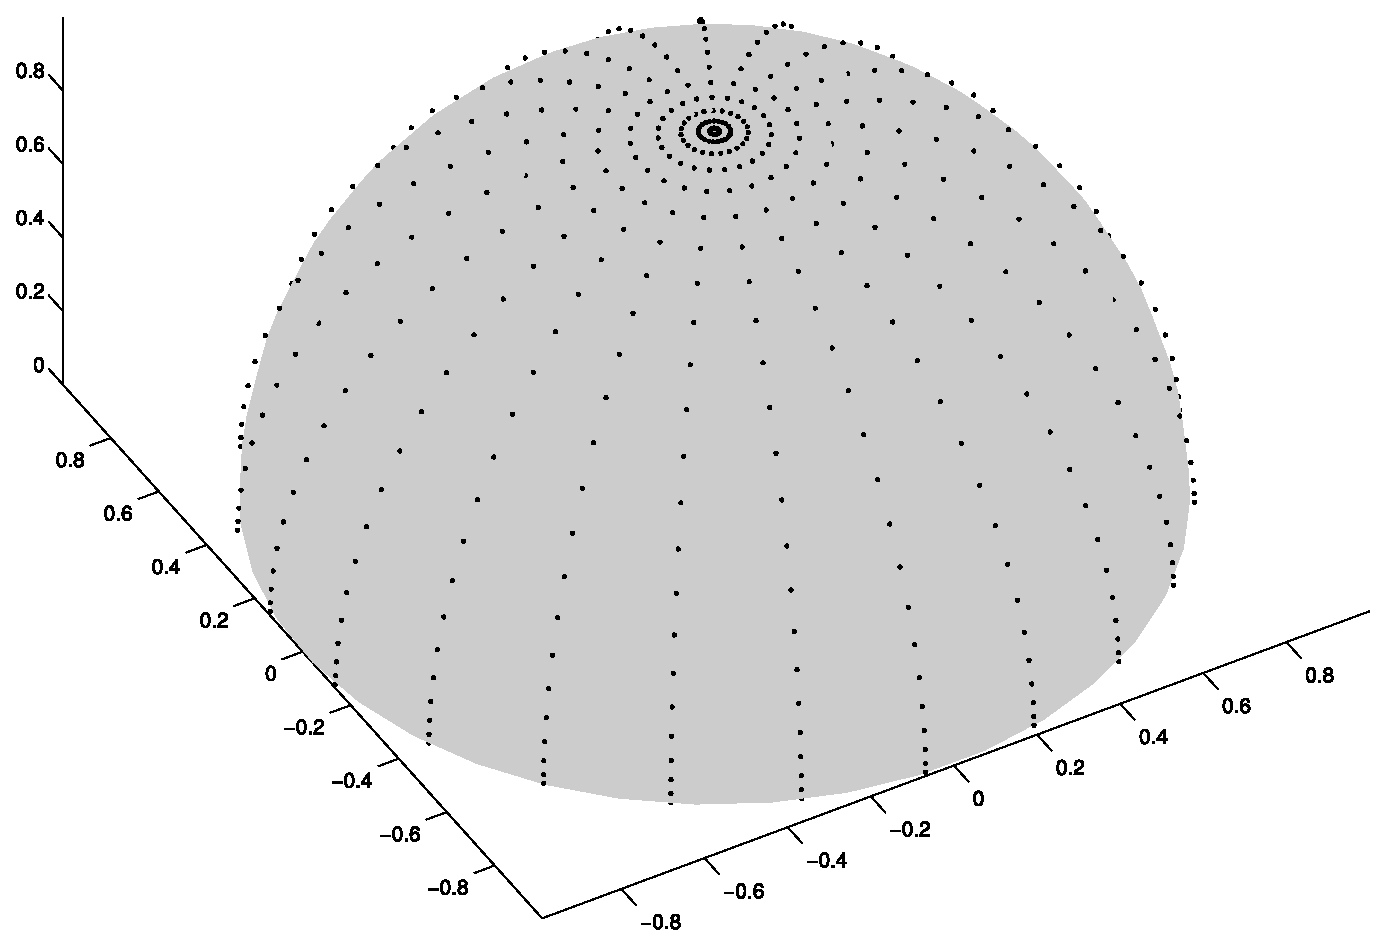
\includegraphics[height=.3\textheight]{quad22mod.eps}
\caption{Расположение узлов квадратуры для полусферы для случая $n = 22$}
\label{fig:quad22}
\end{figure}

\paragraph{Сведение к квадратуре гауссового типа.} Для интеграла
\[
I = \int\limits_0^{\pi/2} S(\cos \theta, \sin \theta) \cos \theta \sin \theta d\theta
\]
сделаем замену переменной $\theta = \frac{\pi}{4} + 2 \arctg \xi$. При этом
\begin{gather*}
r = \cos \theta = \cos \left(\frac{\pi}{4} + 2 \arctg \xi\right) = \frac{1 - 2 \xi - \xi^2}{\sqrt{2}(1 + \xi^2)},\\
z = \sin \theta = \sin \left(\frac{\pi}{4} + 2 \arctg \xi\right) = \frac{1 + 2 \xi - \xi^2}{\sqrt{2}(1 + \xi^2)},\\
Q(r, z) = \frac{W_{2n}(\xi)}{(1 + \xi^2)^n},\qquad d\theta = \frac{2d\xi}{1 + \xi^2},
\end{gather*}
где $W_{2n}(\xi)$ --- многочлен степени не выше $2n$, а сам интеграл принимает вид
\[
I = \int\limits_{1-\sqrt{2}}^{\sqrt{2} - 1}
W_{2n}(\xi) \frac{(1 - \xi^2)^2 - 4\xi^2}{(1 + \xi^2)^{n+3}} d\xi.
\]
Если рассматривать $\omega(\xi) = \frac{(1 - \xi^2)^2 - 4\xi^2}{(1 + \xi^2)^{n+3}} $ в качестве веса, получается классическая задача для построения Гауссовой квадратурной формулы с весом. Для этой задачи разработаны устойчивые вычислительные алгоритмы, например, алгоритм Голуба-Велша \cite{Golub1968}.
Для точного интегрирования многочленов степени $2n$ необходимо и достаточно использовать $n+1$ узел гауссовой квадратуры.
При этом, в силу симметрии весовой функции $\omega(\xi) = \omega(-\xi)$, полученные узлы будут симметричны относительно $\xi = 0$, что гарантирует симметрию $\theta_j = \frac{\pi}{2} - \theta_{n - j}$ для узлов исходной квадратурной формулы.

Хотя задача построения квадратурной формулы для полусферы и может быть сведена к построению гауссовой квадратуры, метод продолжения по параметру был успешно применен для построения и других квадратурных формул, для которых данное сведение не известно.


\section{Решение линейной системы}

Для решения линейной системы \eqref{eq:operator2} применялся метод сопряженных градиентов. Это было обусловлено несколькими факторами:
\begin{itemize}
\item во-первых, так как матрица  $\mathcal A$ системы является положительно определенной и симметричной, метод гарантированно сходится (без учета ошибок округления);
\item во-вторых, для работы метода не требуется знания границ спектра матрицы  $\mathcal A$;
\item в-третьих, метод работает не с матрицей $\mathcal A$ напрямую, а лишь с матрично-векторным произведением  $\mathcal{A} \varphi$;
\item в-четвертых, метод позволяет использовать предобуславливатель для системы.
\end{itemize}

Как было отмечено выше, решение линейной системы соответствует решению дискретизированной системы эллиптических уравнений. Известно \cite{samarskiy}, что эллиптические операторы являются энергетически эквивалентными. Это свойство имеется и у их дискретных аналогов. Если в качестве предобуславливателя для данной задачи взять дискретный аналог некоторой другой системы эллиптических уравнений, то число обусловленности предобусловленной системы, а с ним и количество итераций метода, должно слабо зависеть от мелкости пространственной сетки.

Матрица системы может быть представлена в блочном виде, где каждый блок содержит пространственную дискретизацию некоторого скалярного эллиптического оператора. Пользуясь кронекеровским произведением, объемная часть матрицы $\mathcal{A}$ может быть записана как
\[
\mathcal{A}^\text{объёмн} = \mathscr{H} \otimes M + \sum_{\alpha,\beta} \mathscr{K}^{\alpha\beta} \otimes S_{\alpha,\beta}.
\]
Если из матриц $\mathscr{H}, \mathscr{K}^{\alpha\beta}$ удалить внедиагональные элементы, то полученная матрица
\[
\mathcal{M}^\text{объёмн} = \operatorname{diag}(\mathscr{H}) \otimes M + \sum_{\alpha,\beta}  \operatorname{diag}(\mathscr{K})^{\alpha\beta} \otimes S_{\alpha,\beta}
\]
будет соответствовать некоторой другой системе эллиптических уравнений, энергетически эквивалентной исходной. Заметим, что из-за блочно-диагональной структуры $\mathcal{M}$, она фактически соответствует набору из независимых скалярных эллиптических уравнений. Напротив, матрица $\mathcal{A}$ соответствовала связанной системе эллиптических уравнений.

Другая интерпретация процесса удаления внедиагональных блоков из матрицы $\mathcal{A}$ может быть дана в терминах минимизации функционала $\mathcal{G}$. Если решение системы с матрицей $\mathcal{A}$ эквивалентно решению задачи минимизации \eqref{eq:minimize}
\[
\mathcal{G}(\varphi(\vec r, \vec \Omega)) \to \min_{\varphi(\vec r, \vec \Omega) \in \mathcal{H}_0}
\]
одновременно по всем угловым гармоникам решения $\varphi_k(\vec r)$, то решение системы с матрицей $\mathcal{M}$ соответствует решению задач минимизации
\[
\mathcal{G}(\varphi_{k}(\vec r) \theta_k(\vec \Omega)) \to \min_{\varphi_k(\vec r)}, \quad k = 1, \dots, K.
\]
отдельно для каждой гармоники $\varphi_k(\vec r)$.

\section{Вычисление физических характеристик излучения}

Для вычисления нечетных моментов интенсивности (вектора плотности потока энергии) применяется уравнение
\[
\varkappa_\nu \vec S_\nu + c\div \mathbb T_\nu = \varkappa_\nu \vec S_{\nu,\text{p}}
\]

\section{Реализация метода с использованием графических ускорителей}